\documentclass[preview,tikz]{standalone}
\usepackage{amssymb,amsmath,amsthm,amsfonts}
\usepackage{listings}
\usepackage{tikz}

\usetikzlibrary{backgrounds}
\usetikzlibrary{calc}
\usetikzlibrary{decorations.pathreplacing}
\usetikzlibrary{fit}
\usetikzlibrary{patterns.meta}
\usetikzlibrary{shapes.geometric}

% Custom colors
\usepackage{color}
\definecolor{deepblue}{rgb}{0,0,0.5}
\definecolor{deepred}{rgb}{0.6,0,0}
\definecolor{deepgreen}{rgb}{0,0.5,0}

% Python style for highlighting
\lstset{
    language=Python,
    basicstyle=\small\ttfamily,
    morekeywords={self, max, min, float},              % Add keywords here
    keywordstyle=\color{deepblue},
    emph={
        __init__,
        __getitem__,
    },          % Custom highlighting
    emphstyle=\color{deepred},    % Custom highlighting style
    stringstyle=\color{deepgreen},
    frame=tb,                         % Any extra options here
    showstringspaces=false,
}

\begin{document}
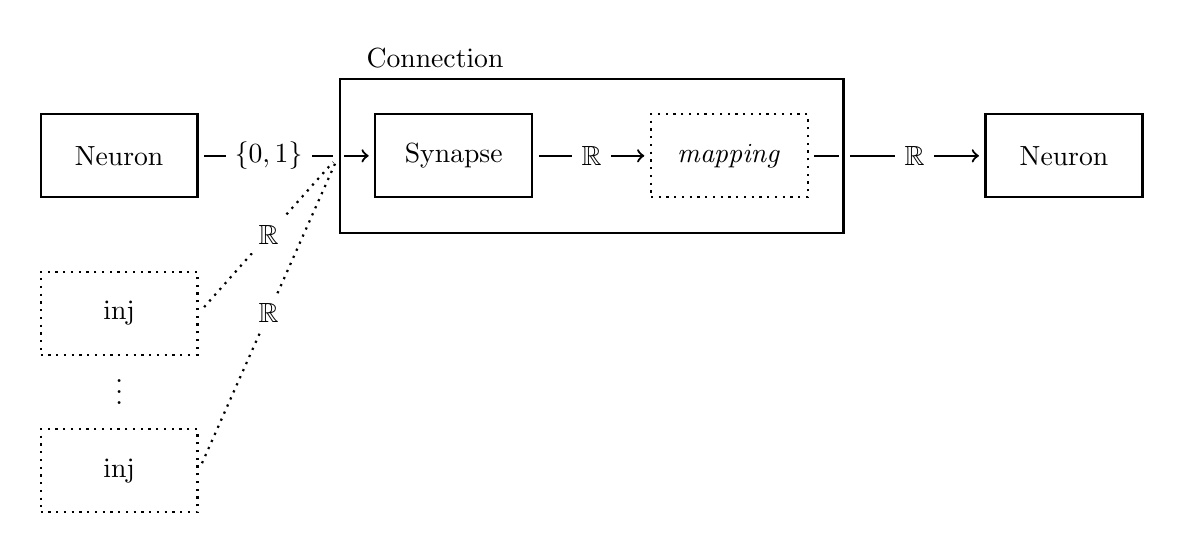
\begin{tikzpicture}[
    background rectangle/.style={fill=white}, show background rectangle,
    component/.style ={rectangle, draw=black, thick, fill=none, text width=5em, text centered, minimum height=3em},
    optional/.style ={rectangle, draw=black, thick, dotted, fill=none, text width=5em, text centered, minimum height=3em},
]
    % extra-connection components
    \node[component] (nin) at (0,0) {\lstinline|Neuron|};
    \node[component] (nou) at (12,0) {\lstinline|Neuron|};
    % connection components
    \node[component] (syn) at (4.25,0) {\lstinline|Synapse|};
    \node[optional] (map) at (7.75,0) {\emph{mapping}};
    \node[rectangle, draw=black, thick, fit=(syn) (map), inner sep=1.25em, label=above left:{\lstinline|Connection|}] (conn) {};
    % inputs
    \node[optional] (ixi) at (0,-2) {inj};
    \node[optional] (ixf) at (0,-4) {inj};
    \node[text centered] (ixdot) at (0, -2.9) {$\vdots$};
    % edges
    \draw[shorten >= 2pt, shorten <= 2pt] (nin) edge[thick] node[midway, fill=white] {$\{0,1\}$} (conn);
    \draw[<-, shorten >= 2pt, shorten <= 2pt] (syn) edge[thick] (conn);
    \draw[->, shorten >= 2pt, shorten <= 2pt] (syn) edge[thick] node[midway, fill=white] {$\mathbb{R}$} (map);
    \draw[shorten >= 2pt, shorten <= 2pt] (map) edge[thick] (conn);
    \draw[->, shorten >= 2pt, shorten <= 2pt] (conn) edge[thick] node[midway, fill=white] {$\mathbb{R}$} (nou);
    \draw[shorten >= 3pt, shorten <= 3pt] (ixi.east) edge[thick, dotted] node[midway, fill=white] {$\mathbb{R}$} (conn.west);
    \draw[shorten >= 3pt, shorten <= 3pt] (ixf.east) edge[thick, dotted] node[midway, fill=white] {$\mathbb{R}$} (conn.west);
\end{tikzpicture}
\end{document}